\section{Principal \texorpdfstring{$\sl_2$}{sl(2)}}

Define $\rho^L \in \at^*$ by $(\rho^L, \alpha_i) = 1$ for all
$\alpha_i \in \Pi$. (Compare with $\rho$, which had $(\rho, \alpha_i\cv) = 1$.)

\begin{exercise}
Show $\rho^L = \frac12\sum_{\alpha \in R^+} \alpha\cv$. In particular, if $R$
is simply laced and normalised so that $(\alpha, \alpha) = 2$, then
$\rho = \rho^L$.
\end{exercise}

Then $(\rho^L, \alpha) = \htt(\alpha) = \sum k_i$ if we write
$\alpha = \sum k_i\alpha_i$.

\begin{exercise}
\[
  F_{\rho^L}(\ch L(\Lambda)) = q^{-(\Lambda, \rho^L)}\prod_{\alpha \in R^+}
    \frac{1 - q^{(\Lambda+\rho, \alpha\cv)}}{1 - q^{(\rho, \alpha\cv)}}.
\]
[\emph{Hint:} apply $F_{\rho^L}$ to the Weyl denominator identity for the
\emph{Langlands dual Lie algebra}, with root system $R\cv$.]
\end{exercise}

Note that $(\lambda + \rho, \alpha\cv)/(\rho, \alpha\cv) = (\lambda + \rho, \alpha)/(\rho, \alpha)$
as $\alpha\cv = 2\alpha/(\alpha, \alpha)$, so we recovered the same formula
for the Weyl dimension.

\begin{definition}
We call $F_{\rho^L}(\ch L(\Lambda))$ the \emph{$q$-dimension} of $L(\Lambda)$,
denoted $\dimq L(\Lambda)$.
\end{definition}

\begin{proposition}
$\dimq L(\Lambda)$ is a unimodal polynomial. More specifically, it lives in
$\N[q, q^{-1}]^{\Z/2}$ or $q^{1/2}\N[q, q^{-1}]^{\Z/2}$ (depending on its
degree), where $\Z/2$ acts by $q \mapsto q^{-1}$, and the coefficients
decrease as the absolute value of the degree gets bigger.
\end{proposition}

\begin{proof}
We will show that $\dimq L(\Lambda)$ is the character of an $\sl_2$-module in
which all ``strings'' have the same parity.

Set $H = 2\nu^{-1}(\rho^L) \in \at \subseteq \g$, and set $E = \sum E_i$.

\begin{exercise}
Check that $[H, E] = 2E$.
\end{exercise}

Writing $H = \sum c_iH_i$ with $c_i \in \C$, set $F = \sum c_iF_i$.

\begin{exercise}\leavevmode
\begin{enumerate}
  \item Show that $E, F, H$ span a copy of $\sl_2$. This is called the
    \emph{principal $\sl_2$}.
  \item Show that if $\Lambda - \gamma$ is a weight of $L(\Lambda)$, then
    $(\Lambda - \gamma, 2\rho^L) \equiv (\Lambda, 2\rho^L) \bmod 2$.
  \item Derive the proposition. (The eigenvalue of $H$ on $L(\Lambda)_\lambda$
    is $(\lambda, 2\rho^L)$, twice the exponent of $q^{-1}$ in
    $F_{\rho^L}(e^\lambda)$.) \qedhere
\end{enumerate}
\end{exercise}
\end{proof}

\begin{exercise}
Write $[n] = (q^n - 1)/(q - 1)$, and $[n]! = [n][n-1]\cdots[1]$. Show that the
following polynomials are unimodal:
\[
  \begin{bmatrix} n \\ k \end{bmatrix} = \frac{[n]!}{[k]!\,[n-k]!}, \qquad
  (1 + q)(1 + q^2)\cdots(1 + q^n).
\]
[\emph{Hint:} for the first, apply the above arguments to $\g = \sl_n$ and
$V = \Lambda^k\C^n$, or to $\g = \sl_{n-k+1}$ and $V = S^k\C^{n-k+1}$. For
the second, apply it to the spin representation of $B_n = \so_{2n+1}$; we will
define the spin representation next time.]
\end{exercise}

\begin{remark}
When is $L(\lambda) \cong L(\lambda)^*$? Precisely when the lowest weight of
$L(\lambda)$ is $-\lambda$. The lowest weight of $L(\lambda)$ is $w_0\lambda$,
where $w_0$ is the (unique) maximal-length element of $W$, which sends all the
positive roots to negative ones.

Now, for a representation $V$ which is isomorphic to its dual $V^*$, we get a
nondegenerate invariant bilinear form on $V$. If $V$ is irreducible, this
bilinear form is either symmetric or antisymmetric. By the above, we see that
we can determine which it is by laboriously computing characters; but can we
tell simply by looking at $\lambda$?

The answer turns out to be yes. Indeed, the form will pair the highest-weight
and the lowest-weight vector, and if we look at the principal $\sl_2$, it is a
string from the highest-weight to the lowest-weight vector. Now, on the
principal $\sl_2$ it is quite easy to see that the form is antisymmetric if the
representation is $L(n)$ with $n$ odd, and symmetric if it is $L(n)$ with $n$
even. Thus, all we need to know is (the parity of) $(\lambda, 2\rho^L)$. This
is called the \emph{Schur indicator}.
\end{remark}

\lecture{22}

\begin{exercise}
Compute $\dimq L(\theta)$, where $L(\theta)$ is the adjoint representation, for
$G_2$, $A_2$, and $B_2$. Then do it for all the classical groups. You will
notice that $L(\theta)|_{\text{principal } \sl_2} = L(2e_1) + \dots + L(2e_l)$,
where $l = \rank \g = \dim \at$, $e_1, \dots, e_l \in \N$, and $e_1 = 1$. The
$e_i$ are called the \emph{exponents of the Weyl group}, and the order of the
Weyl group is $|W| = (e_1 + 1)\cdots(e_l + 1)$. Compute $|W|$ for $E_8$.
\end{exercise}

\section{Crystals}

Let $\g$ be a semisimple Lie algebra, $\Pi = \{\alpha_1, \dots, \alpha_l\}$ the
simple roots, and $P$ the weight lattice.

\begin{definition}
A \emph{crystal} is a set $B$, $0 \notin B$, together with functions
$\wt\colon B \to P$, $\te_i\colon B \to B \sqcup \{0\}$,
$\tf_i\colon B \to B \sqcup \{0\}$ such that
\begin{enumerate}
  \item if $\te_ib \neq 0$, then $\wt(\te_i(b)) = \wt(b) + \alpha_i$; if
    $\tf_ib \neq 0$, then $\wt(\tf_i(b)) = \wt(b) - \alpha_i$;
  \item for $b, b' \in B$, $\te_ib = b'$ if and only if $b = \tf_ib'$;
  \item before we state the third defining property, we need to introduce
    slightly more notation.
\end{enumerate}
\end{definition}

We can draw $B$ as a graph. The vertices are $b \in B$, and the edges are
$b \xrightarrow[i]{} b'$ if $\tf_ib = b'$ (equivalently, $\te_ib' = b$). We say
that this edge is ``coloured by $i$''. This graph is known as the
\emph{crystal graph}.

\begin{example}
In $\sl_2$ the string
\[
  n \to n - 2 \to n - 4 \to \dots \to -n
\]
is a crystal, where the weight of vertex $i$ is $i\alpha/2$.
\end{example}

Define $\epsilon_i(b) = \max\setc{n \geq 0}{\te_i^n(b) \neq 0}$, and
$\phi_i(b) = \max\setc{n \geq 0}{\tf_i^n(b) \neq 0}$:
\[
\begin{tikzpicture}[baseline=-3pt,x=0.9cm]
  \foreach \i in {0,1,2} \node[dot] (p\i) at (\i,0) {};
  \node (b) at (3,0) {$b$};
  \node (d) at (4.2,0) {$\cdots$};
  \node[dot] (q) at (5.4,0) {};
  \node[dot] (r) at (6.4,0) {};
  \draw[->] (p0)--(p1); \draw[->] (p1)--(p2); \draw[->] (p2)--(b);
  \draw[->] (b)--(d); \draw[->] (d)--(q); \draw[->] (q)--(r);
  \draw[decorate,decoration={brace,mirror,amplitude=4pt}] (-0.1,-0.3) -- (2.9,-0.3)
    node[midway,below=4pt] {$\epsilon_i(b)$};
  \draw[decorate,decoration={brace,mirror,amplitude=4pt}] (3.1,-0.3) -- (6.5,-0.3)
    node[midway,below=4pt] {$\phi_i(b)$};
\end{tikzpicture}
\]
In $\sl_2$, the sum $\epsilon_i(b) + \phi_i(b)$ is the length of the string
(the number of arrows in it). On the other hand, if we are in the
highest-weight representation $L(n) = L(n\omega)$ and $\wt(b) = n - 2k$, then
$\epsilon(b) = k$ and $\phi(b) = n - k$, i.e.\
$\phi(b) - \epsilon(b) = (\wt(b), \alpha\cv)$. The third defining property of
crystals is that this happens in general:
\begin{enumerate}[start=3]
  \item $\phi_i(b) - \epsilon_i(b) = (\wt(b), \alpha_i\cv)$ for all
    $\alpha_i \in \Pi$.
\end{enumerate}
Define $B_\mu = \setc{b \in B}{\wt(b) = \mu}$.

\begin{definition}
For crystals $B_1$ and $B_2$, we define the tensor product $B_1 \otimes B_2$ as
follows: as a set, $B_1 \otimes B_2 = B_1 \times B_2$,
$\wt(b_1 \otimes b_2) = \wt(b_1) + \wt(b_2)$, and
\begin{align*}
  \te_i(b_1 \otimes b_2) &= \begin{cases}
    (\te_ib_1) \otimes b_2, & \text{if } \phi_i(b_1) \geq \epsilon_i(b_2),\\
    b_1 \otimes (\te_ib_2), & \text{if } \phi_i(b_1) < \epsilon_i(b_2),
  \end{cases}\\
  \tf_i(b_1 \otimes b_2) &= \begin{cases}
    (\tf_ib_1) \otimes b_2, & \text{if } \phi_i(b_1) > \epsilon_i(b_2),\\
    b_1 \otimes (\tf_ib_2), & \text{if } \phi_i(b_1) \leq \epsilon_i(b_2),
  \end{cases}
\end{align*}
where $b \otimes 0 = 0 \otimes b = 0$.
\end{definition}

That is, we are trying to recreate the picture in figure~\ref{fig:crystal-sl2-again}
in each colour.

\begin{exercise}
Check that $B_1 \otimes B_2$ as defined above is a crystal.
\end{exercise}

\begin{exercise}
$B_1 \otimes (B_2 \otimes B_3) \cong (B_1 \otimes B_2) \otimes B_3$ via
$b_1 \otimes (b_2 \otimes b_3) \mapsto (b_1 \otimes b_2) \otimes b_3$.
\end{exercise}

\begin{figure}[!htbp]
  \centering
  \slcrystal
  \caption{Crystal for $\sl_2$ (as in figure~\ref{fig:crystal-sl2}).}
  \label{fig:crystal-sl2-again}
\end{figure}

\begin{remark}
As we see above, the tensor product is associative. In general, however, it is
not commutative.
\end{remark}

\begin{definition}
$B\cv$ is the crystal obtained from $B$ by reversing the arrows. That is,
$B\cv = \setc{b\cv}{b \in B}$, $\wt(b\cv) = -\wt(b)$,
$\epsilon_i(b\cv) = \phi_i(b)$ (and vice versa), and
$\te_i(b\cv) = (\tf_ib)\cv$ (and vice versa).
\end{definition}

\begin{exercise}
$(B_1 \otimes B_2)\cv = B_2\cv \otimes B_1\cv$.
\end{exercise}

\begin{remark}
We will see in a moment precisely how we can attach a crystal to the basis of a
representation. If $B$ parametrises a basis for $V$, then $B\cv$ parametrises a
basis for $V^*$. The condition on the weights can be seen by noting that if
$L(\lambda)$ has highest weight $\lambda$, then $L(\lambda)^*$ has lowest
weight $-\lambda$.
\end{remark}

\begin{theorem}[Kashiwara]
Let $L(\lambda)$ be an irreducible highest-weight representation with highest
weight $\lambda \in P^+$. Then
\begin{enumerate}
  \item There exists a crystal $B(\lambda)$ whose elements are in one-to-one
    correspondence with a basis of $L(\lambda)$, and the elements of
    $B(\lambda)_\mu$ parametrise a basis of $L(\lambda)_\mu$, so that
    \[
      \ch L(\lambda) = \sum_{b \in B(\lambda)} e^{\wt(b)}.
    \]
  \item For any simple root $\alpha_i$ (i.e.\ a simple $\sl_2 \subseteq \g$),
    the decomposition of $L(\lambda)$ as an $(\sl_2)_i$-module is given by the
    $i$-coloured strings in $B(\lambda)$. (In particular, as an uncoloured
    graph, $B(\lambda)$ is connected, since $L(\lambda)$ is spanned by the
    vectors $(\prod f_i)v_\lambda$.)
  \item $B(\lambda) \otimes B(\mu)$ is the crystal for
    $L(\lambda) \otimes L(\mu)$, i.e.\ $B(\lambda) \otimes B(\mu)$ decomposes
    into connected components in the same way as $L(\lambda) \otimes L(\mu)$
    decomposes into irreducible representations.
\end{enumerate}
\end{theorem}

\begin{remark}
We will mention three proof approaches below. The first of them is due to
Kashiwara, and is in the lecturer's opinion the most instructive.
\end{remark}

\begin{example}
Let $\g = \sl_3$, $V = \C^3 = L(\omega_1)$. We compute $V \otimes V$ and
$V \otimes V^*$; see figure~\ref{fig:crystal-sl3}.
\end{example}

\begin{remark}
Note that while the crystals give the decomposition of the representation
into irreducibles, they do not correspond directly to a basis. That is, there
is no basis compatible with all the $(\sl_2)_i$ that we could use here.
Kashiwara's proof of the theorem uses the \emph{quantum group} $\U_q\g$, which
is an algebra over $\C[q, q^{-1}]$ and a deformation of the universal
enveloping algebra $\U\g$. The two have the same representations, but over
$\C[q, q^{-1}]$ there is a very nice basis which satisfies
$e_ib = \te_ib + q \cdot (\text{some mess})$. Therefore, setting $q = 0$
(``freezing'') will give the crystal.
\end{remark}

\begin{figure}[!htbp]
\centering
\begin{tikzpicture}[x=1.55cm,y=1cm,every node/.append style={font=\small}]
  % V (x) V. Columns: first factor b_1, b_2, b_3; rows: second factor.
  % Black arrows are f_1, red arrows are f_2.
  \foreach \c in {0,1,2} \node[dot] (t\c) at (\c,1.3) {};
  \draw[cr1] (t0)--(t1); \draw[cr2] (t1)--(t2);
  \node[above=1pt] at (t0) {$\omega_1$};
  \node[above=1pt] at (t1) {$\omega_1 - \alpha_1$};
  \node[above=1pt,xshift=10pt] at (t2) {$\omega_1 - \alpha_1 - \alpha_2$};
  \foreach \r in {0,1,2} \node[dot] (l\r) at (-1.1,-\r) {};
  \draw[cr1] (l0)--(l1); \draw[cr2] (l1)--(l2);
  \foreach \r in {0,1,2} \foreach \c in {0,1,2} \node[dot] (g\r\c) at (\c,-\r) {};
  \draw[cr1] (g00)--(g01); \draw[cr2] (g01)--(g02);
  \draw[cr1] (g01)--(g11); \draw[cr1] (g02)--(g12);
  \draw[cr2] (g11)--(g12); \draw[cr2] (g12)--(g22);
  \draw[cr2] (g10)--(g20); \draw[cr1] (g20)--(g21);
  \node[above=1pt,font=\footnotesize] at (g00) {$2\omega_1$};
  \node[left=1pt,font=\footnotesize] at (g10) {$2\omega_1 - \alpha_1$};
  % V (x) V^*
  \begin{scope}[xshift=8.6cm]
  \foreach \c in {0,1,2} \node[dot] (t\c) at (\c,1.3) {};
  \draw[cr1] (t0)--(t1); \draw[cr2] (t1)--(t2);
  \foreach \r in {0,1,2} \node[dot] (l\r) at (-1.1,-\r) {};
  \draw[cr2] (l0)--(l1); \draw[cr1] (l1)--(l2);
  \node[left=1pt,font=\footnotesize] at (l0) {$\alpha_1 + \alpha_2 - \omega_1$};
  \foreach \r in {0,1,2} \foreach \c in {0,1,2} \node[dot] (g\r\c) at (\c,-\r) {};
  \draw[cr1] (g00)--(g01); \draw[cr2] (g01)--(g02);
  \draw[cr2] (g00)--(g10); \draw[cr2] (g02)--(g12);
  \draw[cr1] (g10)--(g11); \draw[cr1] (g11)--(g21);
  \draw[cr1] (g12)--(g22); \draw[cr2] (g21)--(g22);
  \node[above=1pt,font=\footnotesize] at (g00) {$\alpha_1 + \alpha_2$};
  \end{scope}
\end{tikzpicture}
\caption{Crystals for $V \otimes V$ (left) and $V \otimes V^*$ (right), with
$V = \C^3$. The top row is the crystal of the first factor $V$ and the left
column that of the second factor; black arrows are $\tf_1$ and red arrows are
$\tf_2$. Observe $V \otimes V = S^2V + \Lambda^2V = S^2V + V^*$, and
$V \otimes V^* = \C + \sl_3$.}
\label{fig:crystal-sl3}
\end{figure}

Lusztig's proof uses some of the same ideas, where I didn't catch how it goes.

Soon, we will look at Littelmann paths, which give a purely combinatorial way
of proving this theorem (which, on the face of it, is a purely combinatorial
statement).

\begin{definition}
A crystal is called \emph{integrable} if it is the crystal of a highest-weight
module with highest weight $\lambda \in P^+$.
\end{definition}

For two integrable crystals $B_1$, $B_2$, we do in fact have
$B_1 \otimes B_2 \cong B_2 \otimes B_1$ (in general, this is false).

\begin{remark}
There is a combinatorial condition due to Stembridge which determines whether a
crystal is integrable; it is a degeneration of the Serre relations, but we will
not state it precisely.
\end{remark}

\lecture{23} Consider the crystal for the standard representation of $\sl_n$,
$L(\omega_1) = \C^n$:
\[
  e_1 = \omega_1 \xto{1} \omega_1 - \alpha_1 \xto{2} \omega_1 - \alpha_1 - \alpha_2
  \xto{3} \cdots \xto{n-1} \omega_1 - \alpha_1 - \dots - \alpha_{n-1}.
\]
We can use this to construct the crystals for all representations of $\sl_n$
as follows.

Let $\lambda \in P^+$, $\lambda = k_1\omega_1 + \dots + k_{n-1}\omega_{n-1}$.
Then $L(\lambda)$ must be a summand of
$L(\omega_1)^{\otimes k_1} \otimes \dots \otimes L(\omega_{n-1})^{\otimes k_{n-1}}$,
since the highest weight of this representation is $\lambda$ (with
highest-weight vector $\bigotimes v_{\omega_i}^{\otimes k_i}$, where
$v_{\omega_i}$ is the highest-weight vector of $L(\omega_i)$). Moreover,
$L(\omega_i) = \Lambda^i\C^n$ is a summand of $(\C^n)^{\otimes i}$. We
conclude that $L(\lambda)$ occurs in some $(\C^n)^{\otimes N}$ for $N > 0$.
Therefore, the crystal for $\C^n$ together with the rule for taking tensor
products of crystals determines the crystal of every representation of
$\sl_n$.

We introduce the \emph{semi-standard Young tableaux} of a representation. (This
is due to Hodge, Schur, and Young.) Write
\[
  B(\omega_1) = \bx{1} \xto{1} \bx{2} \xto{2} \bx{3} \xto{3} \cdots \xto{n-1} \bx{n}
\]
for the crystal of the standard representation $\C^n$. For $i < n$ let
\[
  b_i = \bx{1} \otimes \bx{2} \otimes \dots \otimes \bx{i} \in B(\omega_1)^{\otimes i}.
\]
(This corresponds to the vector $v_1 \wedge v_2 \wedge \dots \wedge v_i \in \Lambda^i\C^n$,
where the $v_k$ are the basis vectors of $\C^n$.)

\begin{exercise}\leavevmode
\begin{enumerate}
  \item $b_i$ is a highest-weight vector in $B(\omega_1)^{\otimes i}$ of weight
    $\omega_i = e_1 + \dots + e_i$. (Recall that $b \in B$ is a
    highest-weight vector if $\te_ib = 0$ for all $i$.) Hence, the connected
    component of $B(\omega_1)^{\otimes i}$ containing $b_i$ is $B(\omega_i)$.
  \item This connected component $B(\omega_i)$ consists precisely of
    \[
      \setc{\bx{a_1} \otimes \bx{a_2} \otimes \dots \otimes \bx{a_i}}{1 \leq a_1 < \dots < a_i \leq n}
        \subset B(\omega_1)^{\otimes i}.
    \]
\end{enumerate}
\end{exercise}

We write elements of the form
$\bx{a_1} \otimes \bx{a_2} \otimes \dots \otimes \bx{a_i}$ as column vectors
\[
  \begin{array}{|c|} \hline a_1 \\ \hline a_2 \\ \hline \vdots \\ \hline a_i \\ \hline \end{array}\,.
  \qquad\text{For example, the highest weight vector is denoted}\qquad
  \begin{array}{|c|} \hline 1 \\ \hline 2 \\ \hline \vdots \\ \hline i \\ \hline \end{array}\,.
\]

Let $\lambda = \sum k_i\omega_i$. Embed
$B(\lambda) \hookrightarrow B(\omega_1)^{\otimes k_1} \otimes B(\omega_2)^{\otimes k_2}
\otimes \dots \otimes B(\omega_{n-1})^{\otimes k_{n-1}}$ by mapping the highest
weight vector
$b_\lambda \mapsto b_1^{\otimes k_1} \otimes \dots \otimes b_{n-1}^{\otimes k_{n-1}}$
(which is a highest-weight vector in the image). Now, we can represent any
element in
$B(\omega_1)^{\otimes k_1} \otimes \dots \otimes B(\omega_{n-1})^{\otimes k_{n-1}}$
by a sequence of column vectors as in figure~\ref{fig:tableau}, where the
entries in the boxes are strictly increasing down columns and the columns are
placed side by side with the tensor factors read from right to left.

\begin{figure}[!htbp]
\centering
\begin{tikzpicture}[x=0.5cm,y=0.34cm,every node/.append style={font=\small}]
  % columns of height 7 (k_{n-1} = 3), 6 (k_{n-2} = 2), 5 (k_{n-3} = 1),
  % ..., 2 (k_2 = 4), 1 (k_1 = 3); long columns on the left
  \foreach \c/\h in {0/7,1/7,2/7,3/6,4/6,5/5} \draw (\c,0) rectangle (\c+1,-\h);
  \node at (7.5,-0.5) {$\cdots$};
  \foreach \c/\h in {10/2,11/2,12/2,13/2,14/1,15/1,16/1} \draw (\c,0) rectangle (\c+1,-\h);
  \node[left] at (-0.3,-3.5) {$n - 1$};
  \foreach \a/\b/\lab/\d in {0/3/{k_{n-1}}/3pt,3/5/{k_{n-2}}/3pt,5/6/{k_{n-3}}/13pt,10/14/{k_2}/3pt,14/17/{k_1}/3pt}
    \draw[decorate,decoration={brace,mirror,amplitude=3pt}] (\a+0.05,-7.5) -- (\b-0.05,-7.5)
      node[midway,below=\d] {$\lab$};
\end{tikzpicture}
\caption{Generic element of
$B(\omega_1)^{\otimes k_1} \otimes \dots \otimes B(\omega_{n-1})^{\otimes k_{n-1}}$,
a.k.a.\ a semi-standard Young tableau. Here $k_{n-1} = 3$, $k_{n-2} = 2$,
$k_{n-3} = 1, \dots, k_2 = 4$, $k_1 = 3$.}
\label{fig:tableau}
\end{figure}

\begin{definition}
A \emph{semi-standard Young tableau of shape $\lambda$} is an array of numbers
with dimensions as above, such that the numbers strictly increase down
columns, and weakly increase along rows from left to right.
\end{definition}

\begin{theorem}[Exercise]\leavevmode
\begin{enumerate}
  \item The connected component of $B(\lambda)$ in
    $B(\omega_1)^{\otimes k_1} \otimes \dots \otimes B(\omega_{n-1})^{\otimes k_{n-1}}$
    consists precisely of the semi-standard Young tableaux of shape $\lambda$.
  \item Describe the action of $\te_i$ and $\tf_i$ explicitly in terms of
    tableaux.
\end{enumerate}
\end{theorem}

We will now construct the Young tableaux for all the classical Lie algebras.

\begin{example}\leavevmode
\begin{itemize}
  \item $\so_{2n+1}$, i.e.\ type $B_n$: for the standard representation
    $\C^{2n+1}$ we have the crystal
    \[
      \bx{1} \xto{1} \bx{2} \xto{2} \bx{3} \xto{3} \cdots \xto{n-1} \bx{n}
      \xto{n} \bx{0} \xto{n} \bx{\overline{n}} \xto{n-1} \cdots \xto{2}
      \bx{\overline{2}} \xto{1} \bx{\overline{1}}.
    \]
  \item $\so_{2n}$ (type $D_n$): the crystal of the standard representation
    $\C^{2n}$ is
    \[
    \begin{tikzpicture}[baseline=-3pt,x=1.25cm,every node/.append style={font=\small}]
      \node (1) at (0,0) {\bx{1}};
      \node (2) at (1,0) {\bx{2}};
      \node (d1) at (2,0) {$\cdots$};
      \node (m) at (3.1,0) {\bx{n-1}};
      \node (n) at (4.2,0.8) {\bx{n}};
      \node (nb) at (4.2,-0.8) {\bx{\overline{n}}};
      \node (mb) at (5.3,0) {\bx{\overline{n-1}}};
      \node (d2) at (6.4,0) {$\cdots$};
      \node (2b) at (7.4,0) {\bx{\overline{2}}};
      \node (1b) at (8.4,0) {\bx{\overline{1}}};
      \draw[->] (1) -- node[below]{\scriptsize $1$} (2);
      \draw[->] (2) -- node[below]{\scriptsize $2$} (d1);
      \draw[->] (d1) -- node[below]{\scriptsize $n-2$} (m);
      \draw[->] (m) -- node[above left=-2pt]{\scriptsize $n-1$} (n);
      \draw[->] (m) -- node[below left=-2pt]{\scriptsize $n$} (nb);
      \draw[->] (n) -- node[above right=-2pt]{\scriptsize $n$} (mb);
      \draw[->] (nb) -- node[below right=-2pt]{\scriptsize $n-1$} (mb);
      \draw[->] (mb) -- node[below]{\scriptsize $n-2$} (d2);
      \draw[->] (d2) -- node[below]{\scriptsize $2$} (2b);
      \draw[->] (2b) -- node[below]{\scriptsize $1$} (1b);
    \end{tikzpicture}
    \]
  \item $\spl_{2n}$ (type $C_n$): the crystal of the standard representation
    $\C^{2n}$ is
    \[
      \bx{1} \xto{1} \bx{2} \xto{2} \cdots \xto{n-1} \bx{n} \xto{n}
      \bx{\overline{n}} \xto{n-1} \cdots \xto{2} \bx{\overline{2}} \xto{1}
      \bx{\overline{1}}.
    \]
\end{itemize}
\end{example}

\begin{exercise}\leavevmode
\begin{enumerate}
  \item Check that the crystals of the standard representations are as
    claimed.
  \item What subcategory of the category of representations of $\g$ do these
    representations generate?

    Consider the highest weight $\lambda$ of the standard representation. This
    gives an element $\overline{\lambda} \in P/Q$, a finite group dual to
    $Z(G)$ (where $G$ is the simply connected Lie group attached to $\g$).
    Consider the subgroup $\langle\overline{\lambda}\rangle \leq P/Q$. We
    cannot obtain all of the representations unless $P/Q$ is cyclic and
    generated by $\overline{\lambda}$. For the classical examples we have
    $P/Q = \Z/2 \times \Z/2$ for $D_{2n}$, $\Z/4$ for $D_{2n+1}$, and $\Z/2$
    for $B_n$ and $C_n$.
  \item (Optional) Write down a combinatorial set like Young tableaux that is
    the crystal of $B(\lambda)$ with $\lambda$ obtained from the standard
    representation.
\end{enumerate}
\end{exercise}

For $B_n$ we have one more representation, the \emph{spin representation}.
Recall the Dynkin diagram for $B_n$,
\[
\begin{tikzpicture}[baseline=-3pt,x=1.15cm,every node/.append style={font=\small}]
  \node[node] (b1) at (0,0) {}; \node[node] (b2) at (1,0) {};
  \node[node] (b3) at (3,0) {}; \node[node] (b4) at (4,0) {};
  \draw (b1)--(b2); \draw[dotted] (b2)--(b3); \dbond{b3}{b4}
  \node[node] at (b3) {}; \node[node] at (b4) {};
  \node[above=3pt] at (b3) {$e_{n-1} - e_n$}; \node[right=4pt] at (b4) {$e_n$};
\end{tikzpicture}
\]

\begin{definition}
Let $\omega_1, \dots, \omega_n$ be the dual basis to
$\alpha_1\cv, \dots, \alpha_n\cv$. We call $L(\omega_n)$ the \emph{spin
representation}.
\end{definition}

\begin{exercise}
Use the Weyl dimension formula to show that $\dim L(\omega_n) = 2^n$.
\end{exercise}

Define $B = \setc{(i_1, \dots, i_n)}{i_j = \pm 1}$ with
$\wt((i_1, \dots, i_n)) = \frac12\sum i_je_j \in P$, and
\[
  \te_j(i_1, \dots, i_n) = \begin{cases}
    (i_1, \dots, +1_j, -1_{j+1}, \dots, i_n), & \text{if } (i_j, i_{j+1}) = (-1, +1),\\
    0, & \text{otherwise},
  \end{cases}
  \qquad 1 \leq j \leq n - 1,
\]
and
\[
  \te_n(i_1, \dots, i_n) = \begin{cases}
    (i_1, \dots, i_{n-1}, +1), & \text{if } i_n = -1,\\
    0, & \text{otherwise}
  \end{cases}
\]
(note that in particular $\te_i^2 = 0$ always).

\begin{claim}
This is the crystal of the spin representation $L(\omega_n)$.
\end{claim}

\begin{remark}
Note that $\dim L(\omega_n) = \dim \Lambda^\bullet\C^n$. This is for a very good
reason. Indeed, $\gl_n \subset \so_{2n+1}$ via
\[
  A \mapsto \begin{pmatrix} A & & \\ & 0 & \\ & & -JA^TJ^{-1} \end{pmatrix},
\]
and $L(\omega_n)|_{\gl_n} = \Lambda^\bullet\C^n$ (up to a twist by a
one-dimensional character).
\end{remark}

\begin{exercise}
Check that $B|_{\gl_n}$ is the crystal of $\Lambda^\bullet\C^n$.
\end{exercise}

For type $D_n$, the situation is more complicated. We can define
representations
\[
  V^+ = L(\omega_n), \qquad V^- = L(\omega_{n-1});
\]
these are called the \emph{half-spin} representations. The corresponding
crystals are $B^\pm = \setc{(i_1, \dots, i_n)}{i_j = \pm 1}$ with
$\prod i_j = 1$ for $B^+$ and $\prod i_j = -1$ for $B^-$. We define the weight
and most $\te_i$, $\tf_i$ as before, with the change that
\[
  \te_n(i_1, \dots, i_n) = \begin{cases}
    (i_1, \dots, i_{n-2}, +1, +1), & \text{if } (i_{n-1}, i_n) = (-1, -1),\\
    0, & \text{otherwise}.
  \end{cases}
\]

\lecture{24}

\section{Littelmann paths}

Set $P_\R = P \otimes_\Z \R$. By a \emph{path} we mean a piecewise linear
continuous map $[0, 1] \to P_\R$. We consider paths up to
reparametrisation, i.e.\ $\pi \cong \pi \circ \phi$, where
$\phi\colon [0, 1] \to [0, 1]$ is a piecewise-linear isomorphism. (That is, we
care about the trajectory, not about the speed at which we traverse the path.)

Let $\mathcal{P} = \setc{\text{paths } \pi}{\pi(0) = 0,\ \pi(1) \in P}$. Define
a crystal structure on $\mathcal{P}$ as follows: we set
\[
  \wt(\pi) = \pi(1).
\]
To define $\te_i(\pi)$, let
\[
  h_i = \min\Bigl(\Z \cap \setc{\ip{\pi(t)}{\alpha_i\cv}}{0 \leq t \leq 1}\Bigr) \leq 0.
\]
That is, $h_i$ is the smallest integer in the range of
$t \mapsto \ip{\pi(t)}{\alpha_i\cv}$ (note that since $\pi(0) = 0$, we have
$h_i \leq 0$).

If $h_i = 0$, we set $\te_i(\pi) = 0$ (this is not the path that stays at $0$,
but rather the extra element of the crystal).

If $h_i < 0$, take the smallest $t_1 > 0$ such that
$\ip{\pi(t_1)}{\alpha_i\cv} = h_i$. Then take the largest $t_0 < t_1$ such
that $\ip{\pi(t_0)}{\alpha_i\cv} = h_i + 1$.

The idea is to reflect the segment of the path $\pi$ from $t_0$ to $t_1$ in
the hyperplane $\ip{\lambda}{\alpha_i\cv} = h_i + 1$. Therefore, we define the
path $\te_i(\pi)$ as follows (see figure~\ref{fig:littelmann}):
\[
  \te_i(\pi)(t) = \begin{cases}
    \pi(t), & 0 \leq t \leq t_0,\\
    \pi(t_0) + s_{\alpha_i}(\pi(t) - \pi(t_0))
      = \pi(t) - \ip{\pi(t) - \pi(t_0)}{\alpha_i\cv}\alpha_i, & t_0 \leq t \leq t_1,\\
    \pi(t) + \alpha_i, & t \geq t_1.
  \end{cases}
\]

\begin{figure}[!htbp]
\centering
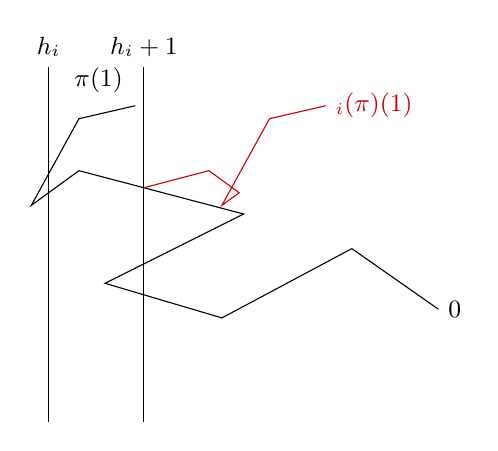
\begin{tikzpicture}[scale=1.1,every node/.append style={font=\small}]
  \draw (0,-2.2) -- (0,1.9) node[above] {$h_i$};
  \draw (1.1,-2.2) -- (1.1,1.9) node[above] {$h_i + 1$};
  % pi, traversed from 0 (bottom right) to pi(1)
  \coordinate (O) at (4.5,-0.9);
  \draw (O) -- (3.5,-0.2) -- (2.0,-1.0) -- (0.65,-0.6) -- (2.25,0.2) -- (0.35,0.7)
        -- (-0.2,0.3) -- (0.35,1.3) -- (1.0,1.45);
  \node[right] at (O) {$0$};
  \node[above left=1pt] at (1.0,1.45) {$\pi(1)$};
  % e_i(pi): reflect the stretch between the last visit to h_i+1 and the
  % first visit to h_i in the line h_i+1, then translate the rest by alpha_i
  % pi meets h_i + 1 for the last time before t_1 at (1.1, 0.503) and first
  % meets h_i at (0, 0.445); alpha_i is drawn as the horizontal vector (2.2, 0)
  \draw[red!80!black] (1.1,0.503) -- (1.85,0.7) -- (2.2,0.445) -- (2.0,0.3)
        -- (2.55,1.3) -- (3.2,1.45);
  \node[red!80!black,right] at (3.2,1.45) {$\te_i(\pi)(1)$};
\end{tikzpicture}
\caption{$\pi$ is drawn in black; $\te_i(\pi)$, from the point where it
deviates from $\pi$, is drawn in red. The vertical lines are the hyperplanes
$\ip{\lambda}{\alpha_i\cv} = h_i$ and $h_i + 1$.}
\label{fig:littelmann}
\end{figure}

\begin{exercise}
Show that $\epsilon_i(\pi) = -h_i$.
\end{exercise}

\begin{example}
Let's compute the crystals of some representations of $\sl_2$. Writing a
straight path by its endpoints,
\[
  \te(0 \to -\alpha/2) = (0 \to \alpha/2), \qquad \te(0 \to \alpha/2) = 0,
\]
and
\[
  \te(0 \to -\alpha) = (0 \to -\alpha/2 \to 0), \qquad
  \te(0 \to -\alpha/2 \to 0) = (0 \to \alpha/2 \to \alpha).
\]
\end{example}

If $\pi$ is a path, let $\pi\cv$ be the reversed path, i.e.\
$t \mapsto \pi(1 - t) - \pi(1)$. Define
\[
  \tf_i(\pi) = \bigl(\te_i(\pi\cv)\bigr)\cv.
\]

\begin{exercise}
With the above definitions, $\mathcal{P}$ is a crystal.
\end{exercise}

Define
$\mathcal{P}^+ = \setc{\text{paths } \pi}{\pi([0, 1]) \subset P_\R^+}$, where
$P_\R^+ = \setc{x \in P_\R}{\ip{x}{\alpha_i\cv} \geq 0 \text{ for all } i}$.
If $\pi \in \mathcal{P}^+$, then $\te_i(\pi) = 0$ for all $i$.

For $\pi \in \mathcal{P}^+$ let $B_\pi$ be the subcrystal of $\mathcal{P}$
generated by $\pi$ (i.e.\ $B_\pi = \{\tf_{i_1}\tf_{i_2}\cdots\tf_{i_r}\pi\} \setminus \{0\}$).

\begin{theorem}[Littelmann]\leavevmode
\begin{enumerate}
  \item If $\pi, \pi' \in \mathcal{P}^+$ then $B_\pi \cong B_{\pi'}$ as
    crystals iff $\pi(1) = \pi'(1)$.
  \item There is a unique isomorphism between this crystal and
    $B(\pi(1))$, the crystal of the irreducible representation
    $L(\pi(1))$. (Of course, the isomorphism sends $\pi$ to the highest-weight
    element of $B(\pi(1))$.)
  \item Moreover, for the path $\pi(t) = \lambda t$, $\lambda \in P^+$,
    Littelmann gives an explicit combinatorial description of the paths in
    $B_\pi$.
\end{enumerate}
\end{theorem}

\begin{example}
Let's compute part of the crystal of the adjoint representation of $\sl_3$,
with simple roots $\alpha$, $\beta$:
\[
  \te_\beta\bigl(0 \to -(\alpha + \beta)\bigr) = (0 \to -\alpha).
\]
\end{example}

\begin{exercise}
Compute the rest of the crystal, and check that you get the adjoint
representation of $\sl_3$.
\end{exercise}

The simplest nontrivial example is $G_2$, the automorphisms of the octonions.

\begin{exercise}
Compute the crystal of the $7$-dimensional and the $14$-dimensional (adjoint)
representations of $G_2$. Compute their tensor product.
\end{exercise}

The tensor product of crystals has a very nice (and natural!) realisation in
terms of concatenating paths:

\begin{definition}
For $\pi_1, \pi_2 \in \mathcal{P}$, define $\pi_1 * \pi_2$ to be the
concatenation (traverse $\pi_1$, then translate $\pi_2$ to start at
$\pi_1(1)$ and traverse it).
\end{definition}

\begin{exercise}
$*\colon \mathcal{P} \otimes \mathcal{P} \to \mathcal{P}$ is a morphism of
crystals.
\end{exercise}

That is, the tensor product of two crystals simply consists of the
concatenated paths in them.

\begin{remark}
We have now defined $B(\lambda)$ explicitly without using $L(\lambda)$. One
can prove the Weyl character formula
\[
  \ch B(\lambda) = \frac{\sum_{w \in W} \det w \, e^{w(\lambda+\rho) - \rho}}{\prod_{\alpha \in R^+} (1 - e^{-\alpha})}
\]
from this, without referring to $L(\lambda)$ or quantum groups. To do this, one
builds $\ch L(\lambda)$ and $L(\lambda)$ itself one root at a time, and uses
the \emph{Demazure character formula}.

More specifically: for each $w \in W$ consider $L_w(\lambda)$, the
$\fn^+$-submodule of $L(\lambda)$ generated by $v_{w\lambda}$, where $v_\lambda$
is the highest weight vector and $v_{w\lambda}$ spans the line
$L(\lambda)_{w\lambda}$. (Equivalently, it is the submodule generated by the
$1$-dimensional space $wL(\lambda)_\lambda$.)
\end{remark}

\begin{theorem}[Demazure character formula]
\[
  \ch L_w(\lambda) = D_w(e^\lambda),
\]
where we write $w = s_{i_1}\cdots s_{i_r}$, a reduced (i.e.\ shortest)
decomposition, and set
\[
  D_w = D_{s_{i_1}}\cdots D_{s_{i_r}}, \qquad
  D_{s_i}(f) = \frac{f - e^{-\alpha_i}s_i(f)}{1 - e^{-\alpha_i}}
    = (1 + s_i)\frac{f}{1 - e^{-\alpha_i}}
    = \frac{f e^{\alpha_i/2} - s_i(f e^{\alpha_i/2})}{e^{\alpha_i/2} - e^{-\alpha_i/2}}.
\]
That is,
\[
  D_{s_i}(e^\lambda) = \begin{cases}
    e^\lambda + e^{\lambda - \alpha_i} + \dots + e^{s_i\lambda}, & \ip{\lambda}{\alpha_i\cv} \geq 0,\\
    0, & \ip{\lambda}{\alpha_i\cv} = -1,\\
    -(e^{\lambda + \alpha_i} + \dots + e^{s_i\lambda - \alpha_i}), & \ip{\lambda}{\alpha_i\cv} < -1.
  \end{cases}
\]
\end{theorem}

``I've got about six minutes. Is that enough time to tell you about the
Langlands program?''

Suppose that $G$ is an algebraic group with Lie algebra $\g$ which is
semisimple. For a given $\g$, there is the smallest group $G$ above it,
$G^{\mathrm{ad}} = G/Z_G$ (whose centre is $\{1\}$). There is also the largest
group, $G^{\mathrm{sc}}$, the simply connected cover of $G$, which is still an
algebraic group. We have $\pi_1(G^{\mathrm{ad}}) \cong (P/Q)^*$ and
$Z_{G^{\mathrm{sc}}} \cong (P/Q)^*$, where $(P/Q)^* = \Hom(P/Q, \C^\times)$
is (non-canonically) isomorphic to $P/Q$.

(For example, $SL_n$ is the simply connected group, and $PSL_n$ is the adjoint
group.)

In this course we have studied the category
$\Rep \g = \Rep G^{\mathrm{sc}}$.

Recall that for $G$ a finite group, the number of irreducible representations
is the number of conjugacy classes, but conjugacy classes do not parametrise
the representations. For us, however, the representations are parametrised
by $P^+ \cong P/W$.

It is possible, for $G$ an algebraic group, to define ${}^LG$, the Langlands
dual group, where the Lie algebra $\g$ and the root system $R$ correspond to
$\g\cv$ and $R\cv$ (and in fact the torus and the dual torus will swap in the
dual group).

If we consider the representations of $G(F)$ where $F = \mathbb{F}_q$ or
$F = \C((t))$, these correspond roughly to conjugacy classes of homomorphisms
$\bigl(W(F) \to {}^LG(\C)\bigr)/{}^LG(\C)$, where $W(F)$ is a ``thickening''
of the Galois group of $F$.
